\documentclass[output=paper,colorlinks,citecolor=brown,newtxmath,hidelinks]{langscibook} 
\ChapterDOI{10.5281/zenodo.2545517}

\title{The Russian perfective present in performative utterances} 

\author{Anja Gattnar\affiliation{University of Tübingen}\and  Johanna Heininger\affiliation{University of Tübingen}\lastand  Robin Hörnig\affiliation{University of Tübingen}}

\abstract{This paper aims to show that perfective verbs in Russian can -- contrary to common sense -- be used in performative utterances without lacking the performative meaning of the sentences. In Russian, performative utterances are generally built with an imperfective (\textsc{ipv}) verb in present tense, first person singular or plural. According to the Slavistic literature, the perfective (\textsc{pv}) verb is at most used in marked contexts and with a few selected performative verbs. In our contribution, we will show experimentally that the use of present perfective verbs in performative utterances is considerably more widespread than supposed so far. In two experiments, Russian native speakers located events in time, providing evidence, first, for the temporal interpretation of the sentence depending on the verbal aspect, and second, concerning whether the temporal interpretation differs depending on how much context is given.

\keywords{Russian, verbal aspect, speech act, performative verbs, interpretation, experimental evidence}
}

\begin{document}

\maketitle
\shorttitlerunninghead{The Russian perfective present in performative utterances}
% * <robin.hoernig@uni-tuebingen.de> 2018-12-10T14:58:17.556Z:
%
% ^.

\section{Introduction}

\subsection{General remarks}
Aspect use in \isi{performative} utterances in \ili{Russian} is the core issue of the present paper. We adopt the terminology of \citet{Eckardt2012} and define a \isi{performative} utterance as a sentence that is used to issue a \isi{speech act} by applying a \isi{speech act verb}. Since the \isi{present tense} of the verb is a precondition for a \isi{performative} utterance, the \textsc{ipv} verbal aspect is preferred in \ili{Russian}. However, the Slavistic research literature describes cases where a \isi{performative speech act} is expressed by a \textsc{pv} verb. This is interesting, because the \textsc{pv} aspect is thought of being unable to appear in \isi{present tense}. Example (\ref{ex:eins_a}) shows a sentence expressing an ordinary correct \isi{performative speech act}, whereas the corresponding version (\ref{ex:eins_b}) with \textsc{pv} \textit{predložu} is unacceptable. Example (\ref{ex:zwei}) demonstrates the same mismatch with another \isi{speech act verb}:

\ea\label{ex:eins}
	\ea[]{\label{ex:eins_a}
		\gll Predlagaju otpravit’sja domoj.\\
			propose\textsc{.ipv} go home\\
		\glt ‘I propose to go home.’
	}
	\ex[*]{\label{ex:eins_b}
		\gll Predložu otpravit’sja domoj.\\
			propose\textsc{.pv} go home\\
            \glt Intended: ‘I propose to go home.’
        }
           \z
\z

\ea\label{ex:zwei} Ja bol’še nikogda ne budu krast',\\‘I will not steal any more,’
	\ea[]{\label{ex:zwei_a}
		\gll kljanjus' ot čistogo serdca.\\
			swear\textsc{.ipv} from pure heart\\
		\glt ‘I swear with all my heart.’
	}
	\ex[*]{\label{ex:zwei_b}
		\gll pokljanus' ot čistogo serdca.\\
			swear\textsc{.pv} from pure heart\\
            \glt Intended: ‘I swear with all my heart.’
           }
           \z
\z

\noindent Different from the verbs in (\ref{ex:eins}) and (\ref{ex:zwei}), there are other \isi{speech act} verbs allowing \textsc{pv} aspect, as in (\ref{ex:drei}):

\ea\label{ex:drei}
	\ea[]{\label{ex:drei_a}
		\gll Ja prošu vas govorit' gromko i po očeredi.\\
        	  I ask\textsc{.ipv} you speak loud and by order\\
              \glt ‘I ask you to speak loudly and one by one.’
        }
	\ex[]{\label{ex:drei_b}
		\gll Ja poprošu vas govorit' gromko i po očeredi.\\
        	  I ask\textsc{.pv} you speak loud and by order\\
		\glt ‘I ask you to speak loudly and one by one.’
            }
            \z
\z

\noindent\citet{Dickey2000}, for example, has noticed that for some \isi{speech act} verbs in \isi{performative} utterances both \textsc{ipv} and \textsc{pv} aspect can be used. Thus, his study is limited to some particular verbs like the \textsc{pv} \textit{verba dicendi} \textit{skazatʾ} ʿto tellʾ, \textit{priznatʾsja} ʿto confessʾ, \textit{zametitʾ} ʿto noteʾ, \textit{pribavitʾ} ʿto addʾ, \textit{poprositʾ} ʿto ask forʾ, \textit{povtoritʾ} ʿto repeatʾ, \textit{doložitʾ} ʿto reportʾ \citep[179]{Dickey2000}. In his opinion, some \textsc{pv} \textit{verba dicendi} are not allowed, like \textit{predložitʾ} ʿto proposeʾ and \textit{pokljastʾsja} ʿto swearʾ; see (\ref{ex:eins}) and (\ref{ex:zwei}).

We want to show that \textsc{pv} \isi{speech act} verbs can perform \isi{performative} utterances to a larger extent than previously expected. We do not assume that the \textsc{pv} and \textsc{ipv} \isi{performative} utterances are used interchangeably. In our opinion, a \textsc{pv} \isi{speech act verb} has an influence on the pragmatic interpretation of the \isi{speech act}. We will not investigate interpretation differences in depth in this paper, but rather we want to experimentally establish that both aspects can indeed be used to utter a \isi{performative speech act}. 

In the following, we give a short overview of the \ili{Russian} \isi{aspectual} system (\sectref{sub:eins:2}). Afterwards we explain the peculiarities of \isi{performative speech} acts and how aspect use is related to it (\sectref{sub:eins:3}). Then, the phenomenon of the present \isi{perfective} is described, which has been intensively studied in the Slavistic literature (\sectref{sub:eins:4}). Subsequently, we discuss the present \isi{perfective} in \isi{performative speech} acts and present the relevant literature on \ili{Russian} performatives (\sectref{sub:eins:5}). These theoretical issues are followed by the presentation of two experiments that we have conducted in St. Petersburg in 2016 (\sectref{sct:zwei}). Finally, we discuss our results and give an outlook for future research (\sectref{sct:drei}).

\subsection{The Russian aspectual system and tense} \label{sub:eins:2}

In \ili{Russian}, aspect is a grammaticalized category. Nearly every \ili{Russian} verb has two aspects that are morphologically distinguished and differ in grammatical function: the \isi{imperfective aspect} (\textsc{ipv}) and the \isi{perfective aspect} (\textsc{pv}). These verb pairs are derived by prefixes or suffixes: \textit{pisat'} ‘to write\textsc{.ipv}’ and \textit{\textbf{na}pisat'} ‘to write\textsc{.pv}’; \textit{otkryt'} ‘to open\textsc{.pv}’ and \textit{otkr\textbf{yva}t'} ‘to open\textsc{.ipv}’.\footnote{Other verb pairs are opposed by suffix only: \textit{kričat' -- kriknut'} ‘to cry‘ or by suppletion \textit{brat' -- vzjat'} ‘to take‘. A smaller group of verbs do not form pairs: (i) biaspectual verbs: \textit{kaznit'} ‘to punish’, (ii) \textit{imperfectiva tantum}: \textit{sidet'} ‘to sit’, and (iii) \textit{perfectiva tantum}: \textit{rinut'sja} ‘to pounce on’.} The \textsc{ipv} aspect is used for (i) habitual or iterated actions, (ii) single, incomplete actions in progress, and (iii) actions which do not emphasize the result. The \textsc{pv} aspect is used (i) for  single, completed actions or (ii) ongoing actions intended to be completed.\footnote{There is a huge range of works on verbal aspect and its meaning to which we cannot refer in this paper. Therefore we limited our selection to pure Slavistic or \ili{Russian} works that are generally accepted among Slavists and in \ili{Russian} aspectology: \citet{Anstatt2003,Avilova1976,Bondarko1971,Breu1980,Breu2000ProblemederInteraktion,Comrie1976,Dickey2000,Galton1976,Klein1995,Lehmann1999,Maslov1984,Mehlig1980,Paduceva1996,Petruchina2000,Rassudova1968,Zaliznjak2000}; etc.}

Morphosyntactically there exist only  three tense categories: preterite, present, and future. Not all three categories are represented in both \textsc{ipv} and \textsc{pv} aspect. Whereas \textsc{ipv} verbs conceptualize all three tense categories, \textsc{pv} verbs appear only in preterite and future, because \isi{present tense} is not compatible with the concept of completeness. The lack of \isi{present tense} marking for \textsc{pv} verbs plays a key role in our investigation. \tabref{tab:eins}, a simplified version of \citet{Swan1978}, summarizes the (semantic) categories resulting from crossing aspect with tense in \ili{Russian}.

\begin{table}
\caption{Tense and aspect in Russian}
\label{tab:eins}
 \begin{tabular}{lccl} 
  \lsptoprule
		& {Past} & {Present} & {Future} \\ 
  \midrule
    \textsc{ipv} &  \ding{51} & \ding{51} & \ding{51} (with ‘be’ + \isi{infinitive})\\
    \textsc{pv}  &  \ding{51} & \ding{55} & \ding{51} \\
  \lspbottomrule
 \end{tabular}
\end{table}

\subsection{Performatives}\label{sub:eins:3}

A \isi{speech act} is called \isi{performative} when the utterance and the action named by a \isi{speech act verb} take place simultaneously. The utterance is part of the action \citep{Austin1962} and performs it. Performative utterances are not statements that are true or false, but concrete, unique actions. In \ili{Russian}, by default, performatives are expressed with the \textsc{ipv} aspect present, first person; see examples (\ref{ex:vier})--(\ref{ex:sieben}).

\ea\label{ex:vier}
\gll Obeščaju	tebe	poechat’	k	babuške.\\
      promise\textsc{.ipv} 	you 	go 		to 	grandmother\\
\glt ‘I promise you to go to grandmother.’
\z

\ea\label{ex:sechs}
\gll Blagodarju 		za ponimanie.\\
 	thank\textsc{.ipv} 	for			understanding\\
\glt ‘Thank you for understanding.’
\z

\ea\label{ex:sieben}
\gll Ja očen’ žaleju, čto my ne vstretilis’ s vami.\\
        I   very	apologize\textsc{.ipv}	that	we	not	meet	with	you\\
\glt ‘I deeply apologize, that we didn´t meet you.’
\z

\noindent We share the opinion with \citet{Apresjan1988}, \citet{Paduceva1994}, and \citet{Petruchina2000} that \isi{performative} verbs in \ili{Russian} can only express a punctual event and not a process. They do not describe an ongoing event, because the action expressed by the verb is accomplished once the speaker finishes the utterance \citep{Petruchina2000}. Therefore, it would be incorrect to translate one of the above examples, for instance (\ref{ex:vier}), with the \ili{English} continuous form: \textit{*I am promising you to go to grandmother.}\footnote{\citet{Harnish2007} discusses the \ili{English} present progressive in performatives and shows that \isi{performative} utterances favor the simple present.}

As \textsc{pv} cannot get a \isi{present tense} marking in \ili{Russian}, we would expect that only the \textsc{ipv} \isi{speech act} verbs can be used in \isi{performative speech} acts. However, we have found examples with \textsc{pv} \isi{speech act} verbs in \isi{performative speech} acts, as in (\ref{ex:acht_a}) from the \ili{Russian} National Corpus (RNC):\footnote{Interestingly, \textsc{pv} \isi{speech act} verbs systematically fail the ‘hereby’-test, which is only feasible with \textsc{ipv} verbs: \textit{S ėtim ja prošu[\textsc{ipv}] vas govorit’ gromko.} ‘Hereby I ask you to speak loudly’ vs. \textit{*S ėtim ja poprošu[\textsc{pv}] vas govorit’ gromko} \citep{Eckardt2012}.}

\ea\label{ex:acht}
	\ea[]{\label{ex:acht_a}
		\gll Pozdravim že našich peredovikov i zaodno prezidenta s neverojatnym uspechom!\\
        	  congratulate\textsc{.pv.1pl} \textsc{ptcl} our labor.activists and simultaneously president   with amazing success\\
        }
	\ex[]{\label{ex:acht_b}
		\gll Pozdravljaem že našich peredovikov i zaodno prezidenta s neverojatnym uspechom!\\
        	  congratulate\textsc{.ipv.1pl} \textsc{ptcl} our labor.activists and simultaneously president   with amazing success\\
		\glt ‘We congratulate our labor activists and also the president for the amazing success.’
            }
            \z
\z

\noindent In (\ref{ex:acht_a}) the \textsc{pv} \isi{speech act verb} \textit{pozdravim} ‘congratulate\textsc{.pv.1pl}’ is used to perform a \isi{speech act}. In (\ref{ex:acht_b}) we replaced the \textsc{pv} verb of the original sentence with the corresponding \textsc{ipv} verb \textit{pozdravljaem} ‘congratulate\textsc{.ipv.1pl}’. (\ref{ex:acht_b}) is a properly built \isi{performative} sentence with the \textsc{ipv} verb meeting all three conditions for a successful \isi{performative speech act}: \isi{speech act verb}, first person, and \isi{present tense}. We find it plausible to assume that (\ref{ex:acht_a}) expresses a \isi{performative speech act}, too.

It is interesting for us whether a \textsc{pv} \isi{speech act verb} changes the sentence meaning compared to the corresponding \textsc{ipv} verb, for instance with respect to our variants (\ref{ex:acht_a}) versus (\ref{ex:acht_b}). The occurrence of present \isi{perfective} \isi{speech act} verbs is documented in many works, but we don't know of any experimental investigation addressing the interpretation of \isi{performative} utterances as a function of the verb aspect. Are utterances with \textsc{pv} \isi{speech act} verbs actually understood as \isi{performative speech} acts? If yes, what does this imply for the temporal localization of the event denoted by the \textsc{pv} \isi{speech act verb}? In our study we presuppose that the localization of an event denoted by a \isi{speech act verb} in the present indicates a \isi{performative} interpretation. We feel confident that sentences with \textsc{pv} \isi{speech act} verbs are \isi{performative} utterances only in the case that they express an event that proceeds simultaneously with the utterance time. This is only possible, when the \textsc{pv} \isi{speech act verb} is interpreted as present \isi{perfective}.  

In the next section we will present arguments for a \textsc{pv} in \isi{performative} utterances in \ili{Russian} and invoke the debate on the present \isi{perfective}.

\subsection{The present perfective in Russian}\label{sub:eins:4}

The debate on the present \isi{perfective} started with \citet{Koschmieder1929}. He declares, initially only for \ili{Polish}, that present \isi{perfective} is possible in non-future meaning solely when the action time coincides with the utterance time and when the verb is in first person form. \citet[120]{Forsyth1970} even claims: “Their use in non-future meanings, however, is extremely common and not on the least exceptional." \citet{Svedova1980} supports this view and notes that under certain syntactic conditions the \textsc{pv} verb can denote actions that take place in the present and not in the future with nuances of meaning. \citet{Rathmayr1976} goes even further. She is of the opinion that the present \isi{perfective} is equal to \textsc{ipv} present plus some stylistic function; yet the stylistic properties are difficult to identify: Even if they are identified by a survey of native speakers they are anticipated to strongly diverge. 

\citet{Dickey2000}, as before him \citet{Bondarko1971} and \citet{Galton1976}, calls the phenomenon of present \isi{perfective} “the temporal coincidence of a situation that is referred to a \textsc{pv} present form in the moment of the utterances". The present \isi{perfective} does not refer to the future but to the time of utterance and, simultaneously, to the time at which the action denoted by the \textsc{pv} verb takes place. \citet{Dewit2017} dubs the phenomenon differently, “the present \isi{perfective} paradox”, because the meaning of the temporal localization that belongs to the \textsc{pv} aspect should prevent the use of present \isi{perfective} in \ili{Russian}. Additionally, the occurrence of present \isi{perfective} in \ili{Russian} is explained in terms of the \isi{aspectual} function of the \textsc{pv} aspect. \citet{Dewit2017} agrees with \citet{Breu2000ProblemederInteraktion} who notices that the \isi{aspectual} meaning of the present \isi{perfective} is stronger than the temporal meaning. In present perfectives, the \isi{aspectual} meaning should be stronger than the temporal meaning of the aspect, because the meaning of temporal localization that is expressed by the \textsc{pv} aspect would prevent the use of present \isi{perfective}. We will discuss this view at the end of the paper. 

So far we have argued for the availability of a present \isi{perfective} in \ili{Russian}. But it still remains open, however, what kind of influence \isi{perfective} present has in contexts where it substitutes the \textsc{ipv}. 

\subsection{The range of present perfective in performatives}\label{sub:eins:5}

Like others, we accept the present \isi{perfective} as means of expressions with the above mentioned readings. We argue that the high acceptability of present \isi{perfective} implies that \textsc{pv} \isi{speech act} verbs are able to fulfill a \isi{performative speech act}. This is a purely theoretical assumption and based on the mentioned theoretical works, empirically supported only in a few cases by way of corpus data \citep{Laczinski2014,Wiemer2014}. Before we  present our experimental work, it is necessary to mention some aspects concerning the type of \isi{speech act} verbs that are used in \textsc{ipv} and \textsc{pv} as well as to give possible conceptual differences between the use of \textsc{ipv} and \textsc{pv} \isi{speech act} verbs that are offered in the research literature.

In the Slavistic research literature several works attest the occurrence of \textsc{pv} \isi{speech act} verbs in \isi{performative speech} acts. But the use of \textsc{pv} verbs, according to these works, is limited to special verb types. For example, \citet{Rjabceva1992} and \citet{Dickey2000} claim that only a few \textsc{pv} \textit{verba dicendi} can be used in competition with \textsc{ipv} performatives. Only for those verbs the \textsc{pv} verb may be used and only those \textsc{pv} verbs may perform a \isi{performative} utterance. Contrary to \citeauthor{Rjabceva1992} and \citeauthor{Dickey2000}, \citeauthor{Wiemer2014} shows that the use of \textsc{pv} \isi{speech act} verbs is also possible for some social performatives like request, desire, thanks, refusal and approval, see example (\ref{ex:neun}). \citet{Laczinski2014} agrees with \citeauthor{Wiemer2014} and demonstrates similar corpus data for \ili{Polish}, \ili{Czech} and \ili{Slovak}.

\ea\label{ex:neun}
\gll Ispol’zuja ėti sposoby, uverju čto vam budet legko zanimat’sja russkim jazykom.\\
             using               this         methods,	assure\textsc{.pv}	   that	         you.\textsc{dat}	  will.be        easily          study         \ili{Russian}                 language\\
\glt ‘When you use this methods, I assure that you will easily learn \ili{Russian}.’\\
\hfill \citep[107]{Wiemer2014}
\z

\newpage 
\noindent The corpus findings of \citeauthor{Wiemer2014} and \citeauthor{Laczinski2014} lead us to the question, whether the range of \textsc{pv} verbs in \isi{performative} utterances is wider than \citeauthor{Rjabceva1992} and \citeauthor{Dickey2000} assume. Some more detailed consideration is given by \citet{Israeli1996,Israeli2001}. She classifies \isi{speech act} verbs into three groups depending on the verbal aspect that a \isi{speech act verb} can take to perform a \isi{speech act} \citep[84]{Israeli2001}: (i) verbs performing a \isi{speech act} only with \textsc{ipv} (see (\ref{ex:eins}) and (\ref{ex:zwei})), for example \textit{prikazyvat’} ‘to order\textsc{.ipv}’, \textit{trebovat’} ‘to demand\textsc{.ipv}’, \textit{blagodarit’} ‘to thank\textsc{.ipv}’, \textit{pozdravljat’} ‘to congratulate\textsc{.ipv}’ etc., often the \textsc{ipv} \isi{speech act verb} has an iterative meaning; (ii) verbs performing a \isi{speech act} both with \textsc{ipv} and \textsc{pv} (see (\ref{ex:drei})), for example \textit {prosit’/poprosit’} ‘to request\textsc{.ipv}/\textsc{.pv}’, \textit{sovetovat’/posovetovat’} ‘to advise\textsc{.ipv}/\textsc{.pv}’, želat’/poželat’ ‘to wish\textsc{.ipv}/\textsc{.pv}’, etc.; (iii) verbs performing a \isi{speech act} only with \textsc{pv}; in the latter case, the verb functions as structuring element, like \textit{perejdëm k novoj teme} ‘let’s open\textsc{.pv} a new future topic’, \textit{otmetim} ‘we note\textsc{.pv}’, \textit{zametim} ‘we mention\textsc{.pv}’ etc. (see example (\ref{ex:elf})). 

\ea\label{ex:zehn}
\gll  Govorju tebe -- živ, živ!\\
         say\textsc{.ipv} you {} living, living\\
\glt ‘I'm telling you -- I'm alive, alive!’
\z

\ea\label{ex:elf}
\gll Ja vam bol’še skažu: net povesti pečal’nee na svete.\\
            I   you   say\textsc{.pv}  more: \textsc{neg.}is story sadder in world\\
\glt ‘Even more, there's no sadder story in the world.’
\z

\noindent According to \citet{Israeli2001}, \textsc{ipv} and \textsc{pv} \isi{performative} utterances of the second group cannot be used interchangeably. This makes the \isi{aspectual} competition particularly interesting for us. Although the alleged semantic or pragmatic differences in the interpretation of \textsc{ipv} and \textsc{pv} \isi{speech act} verbs are not the central issue of this paper, we would like to shortly address Israeli’s account. Whereas we believe that her account  provides a promising perspective for future investigation, the first task accomplished here is to provide evidence that \textsc{pv} verbs actually can be used in carrying out a \isi{performative speech act}.\largerpage[2]

Israeli argues that \textsc{ipv} and \textsc{pv} \isi{speech act} verbs differs with respect to authority marking in \isi{performative} utterances. A typical example for the authority marking in \isi{performative} utterances in her sense is seen in (\ref{ex:zwoelf_a}) from the oral corpus of the RNC. According to Israeli, the sentence shows, in comparison with (\ref{ex:zwoelf_b}), how the different aspect use can influence the speaker’s position of authority:

\ea\label{ex:zwoelf} 
	\ea[]{\label{ex:zwoelf_a} \textit{Situation:} Teacher to student:\\
		\gll Ja poprošu vas govorit' gromko i po očeredi.\\
     I  ask\textsc{.pv.1sg} you         speak               loud            and        by          order\\
		\glt ‘I ask you to speak loudly and one by one’\hfill (RNC, oral corpus)
        }
	\ex[]{\label{ex:zwoelf_b} \textit{Situation:} Young man to museum attendant:\\
		\gll Prošu vas nikomu ni zvuka!\\
        	  ask\textsc{.ipv.1sg} you nobody no word\\
		\glt ‘I ask you to tell nobody.’\hfill (RNC, oral corpus)
            }
            \z
\z

\noindent The use of the \textsc{pv} verb \textit{poprosit’} ‘to ask\textsc{.pv} for’ in (\ref{ex:zwoelf_a}) can be connected with the communicative situation. The \textsc{pv} \isi{speech act verb} stresses the authority of the teacher [+authority] towards the student. In (\ref{ex:zwoelf_b}) the \textsc{ipv} verb \textit{prosit’} ‘to ask\textsc{.ipv} for’ is used in a communication between a young man and a museum attendant. We might argue with \citeauthor{Israeli2001} that the \textsc{ipv} verb in (\ref{ex:zwoelf_b}) is pragmatically neutral or even a polite request.\footnote{The examples (\ref{ex:zwoelf_a}) and (\ref{ex:zwoelf_b}) do not only differ in aspect use. In addition, the [+authority] marked utterance (\ref{ex:zwoelf_a}) has an overt subject \textit{ja} ‘I’ whereas in (\ref{ex:zwoelf_b}) there is a null subject. We also agree with one of the reviewers that the sentences improve with overt subject. Our own corpus investigation leads us to the assumption that an overt subject encourages the [+authority] marker. We did not yet test sentences with overt subjects experimentally, but consider it a future task to do so.\label{fn5}} In \sectref{sct:zwei} we will now present our two experiments that give evidence that sentences with a \textsc{pv} \isi{speech act verb} are interpreted as \isi{present tense} utterances. 

\section{Experimental evidence}\label{sct:zwei}

We have provided instances of present \isi{perfective} in \isi{performative speech} acts in \ili{Russian} from the literature as well as from the RNC. The interpretation of the \textsc{pv} speech acts has not yet been demonstrated experimentally. \citet{Rathmayr1976} mentions that she has asked four (sic!) informants and every one of them has given her another interpretation. Others work with their own intuition or support their arguments by presenting examples from corpus investigation \citep{Wiemer2014,Laczinski2014}. The main concern is to study if sentences like (\ref{ex:zwoelf_a}) are interpreted as \isi{performative speech} acts or not. In (\ref{ex:zwoelf_a}) the verb has the grammatical form \textsc{1sg pv} aspect. The additional meaning that refers to the aspect function of \textsc{pv} aspect would be ‘will ask for’. In future meaning the sentence is not a \isi{performative speech act} but a statement about an event in the future: In the future there will be a situation in which I am saying \textit{I ask you to speak loudly and one by one.} Our aim is now to investigate the temporal alignment of \textsc{pv} \isi{performative} verbs in morphological present.

Our assumption is that in \isi{performative} context the use of the present \isi{perfective} is becoming more widespread than it is reflected in the literature so far. We even tend to assume that every \textsc{pv} \isi{speech act verb} can principally be used to execute a \isi{performative speech act}. Our experiments reported below compare the temporal interpretation of \isi{speech act} verbs with \isi{perfective} versus \isi{imperfective aspect}: Are \textsc{pv} \isi{speech act} verbs never or reliably less often interpreted as \isi{present tense} \textsc{ipv} \isi{speech act} verbs? We assume that:

\begin{itemize}
\item A future tense interpretation indicates that the event denoted by the \textsc{pv} verb does not coincide with the time of utterance, that is, the tense is not considered present \isi{perfective} and the sentence is not understood as a \isi{performative speech act}.
\item A \isi{present tense} interpretation indicates that the event denoted by the \textsc{pv} verb coincides with the time of utterance and, therefore, the tense is considered present \isi{perfective}. The \isi{performative} reading is thus available. In the case of \isi{performative} utterances the context can also be a pragmatic \isi{presupposition}. The hearer expects the honesty of the speaker who cares about the success of the rules.
\end{itemize}

The two experiments that are presented in this section test our hypothesis that \textsc{pv} \isi{speech act} verbs used in \isi{performative} utterances may substitute \textsc{ipv} verbs. 

\subsection{Method}

\subsubsection{Participants}

41 native speakers of \ili{Russian} participated in Experiment 1 without \textsc{Stop-reading} (as explained in \sectref{sct:zwei.eins.drei} below), a different sample of 40 \ili{Russian} native speakers took part in Experiment 2 with \textsc{Stop-reading}. All participants were students of Saint Petersburg State University. They were paid 10~{\small\euro} for their participation.

\subsubsection{Material}

20 verbs were selected from a pool of 28 \isi{speech act} verbs, based on acceptability scores gathered in a web-based pilot study:\footnote{43 \ili{Russian} native speakers judged performatives containing the verbs without preceding context on a scale from 0 to 6 (= most acceptable); mean acceptabilities of the 20 selected verbs were $3.7$ (SD $0.96$) and $1.7$ (SD $0.96$) for performatives with \textsc{ipv} and \textsc{pv} verb aspect, respectively.} 
\textit{uverit' / uverjat'} ‘to assure sth. to so’, 
\textit{izvinit'sja / izvinjat'sja} ‘to apologize for sth.’, 
\textit{poprosit' / prosit'} ‘to ask for sth.’, 
\textit{potrebovat' / trebovat'} ‘to demand sth. from so’, 
\textit{poželat' / ženat'} ‘to wish sth. to so.’, 
\textit{poblagodarit' / blagodarit'} ‘to thank so. for sth.’, 
\textit{priznat'sja / priznavat'ja} ‘to admit sth. to so.’, 
\textit{priglašat' / priglasit'} ‘to invite so. to sth.’, 
\textit{razrešit' / razrešat'} ‘to allow so. to do sth.’, 
\textit{objazyvat'sja / objazat'sja} ‘to commit oneself to sth.’, 
\textit{pochvalit' / chvalit'} ‘to praise so. for sth.’, 
\textit{predupredit' / predupreždat'} ‘to warn so. of sth.’, 
\textit{predstavit' / predstavljat'} ‘to introduce so. to so.’, \textit{poprivetstvovat' / privetstvovat'} ‘to welcome so.’, 
\textit{priznat' / priznavat'} ‘to recognize so. as so.’, 
\textit{prikazat' / prikazyvat'} ‘to order so. to do sth.’, 
\textit{otklonit' / otklonjat'} ‘to reject sth.’, 
\textit{pozdravit' / pozdravljat'} ‘to congratulate so. for sth.’, 
\textit{prostit' / proščat'} ‘to forgive sth. to so.’, 
\textit{otkazat' / otkazyvat'} ‘to refuse sth. to so.’

Two variants of a \isi{performative} target sentence (in short: \isi{performative}) were constructed for each verb. The variants differed only in the aspect of the sentence initial verb which was either \isi{imperfective} or \isi{perfective} present in the first person singular, exemplified in (\ref{ex:item_a}) and (\ref{ex:item_b}). Both \isi{performative} variants were preceded by the same context consisting of two or three sentences.\footnote{The complete list of stimuli can be found here: \url{http://hdl.handle.net/11022/0000-0007-CB0A-A@Appendix.pdf}.\label{fn:app}}

\ea\label{ex:item} \textit{Context:} Vere predlagajut novuju dolžnost' na rabote. Ona dolgo kolebletsja, no eë načal'nik govorit:
    \glt `Vera is offered a new position at work. She hesitates for a long time, but her boss says:'
	\ea\label{ex:item_a} 
		 \gll    Uverjaju Vas, čto ėta dolžnost' -- važnyj šag na puti k uspechu.\\
              assure\textsc{.ipv.pres.1sg} you that this position {} great step on way to success\\
	\ex\label{ex:item_b}
		 \gll    Uverju Vas, čto ėta dolžnost' -- važnyj šag na puti k uspechu.\\
              assure\textsc{.pv.pres.1sg} you that this position {} great step on way to success\\
              \z
		\glt ‘I assure you, that this position is a great step towards success.’     
\z

\noindent In addition to the performatives, two variants of non-\isi{performative}, declarative target sentences (in short: declaratives) were constructed for each of the twenty verbs, serving as control items. Again, the target variants differed only in the aspect of the verb which was either \textsc{ipv} or \textsc{pv} past in the third person singular, as exemplified in (\ref{ex:control_a}) and (\ref{ex:control_b}). Both declarative variants were preceded by the same context which differed from the one of the performatives.

\ea\label{ex:control} \textit{Context:} Terapevt zaxodil v palatu k pacientam po utram.
    \glt ‘The therapist came to the patients into the ward in the morning.’
	\ea\label{ex:control_a} 
		 \gll    Vrač uverjal ich v tom, čto oni vse skoro vyzdorovejut.\\
              doctor assure\textsc{.ipv.past.3sg} them at that, that they all soon will.recover\\
	\ex\label{ex:control_b}
		 \gll    Vrač uveril ich v tom, čto oni vse skoro vyzdorovejut.\\
              doctor assure\textsc{.pv.past.3sg} them at that, that they all soon will.recover\\
              \z
		\glt ‘The doctor assured them, that they will all recover soon.’        
\z

\noindent In addition to the performatives and the controls, 40 fillers were added to the material. The two variants of the performatives and the controls were assigned to two lists such that each item variant was assigned to one of the lists and either list contained 10 performatives and 10 controls with \textsc{ipv} and \textsc{pv} aspect. About the same number of participants was tested with either list, hence all participants worked on a set of 80 items consisting of a context followed by a target. 

\subsubsection{Procedure}\label{sct:zwei.eins.drei}

Participants were tested separately in a quiet room at the Laboratory of Cognitive Studies at the State University of Saint Petersburg. Participants were randomly assigned to Experiment 1 without \textsc{Stop-Reading} or Experiment 2 with \textsc{Stop-Reading}. Participants were seated in front of a PC and instructed about the task to be performed. In each experiment participants worked on three practice trials to get familiar with the procedure before they moved on to the experimental block of trials.

In Experiment 1 without \textsc{Stop-Reading}, a trial began with a full presentation of the context. Participants read the context until they understood what happened and then pressed the space bar. Now the context was replaced by the target sentence displayed left-aligned in the centre of the screen. Participants read the target sentence to understand what happened next; their task was to indicate by means of three cursor keys, where the event described in the target sentence was located in time: ‘$\leftarrow$’ $\hat{=}$ past, ‘$\uparrow$’ $\hat{=}$ present, ‘$\rightarrow$’ $\hat{=}$ future (Response 1). For the sake of congruence with Experiment 2, the whole sentence was presented again immediately after Response 1, prompting participants to indicate the location again by pressing one of the cursor keys (Response 2). In order to encourage participants to read the contexts and targets carefully, half of the trials ended with a yes-no comprehension question that was answered by means of two designated keys (mean accuracy: $91\%$). A session lasted for about 20 minutes.

Trials in Experiment 2 with \textsc{Stop-Reading} began with a full presentation of the context, too. Once participants understood what was told in the context they pressed the space bar. Now the context was replaced by the target sentence displayed left-aligned in the centre of the screen, yet masked except for the first word; masked characters other than blanks were substituted by underscores. Participants could then read the target sentence from left to right in a word by word fashion (moving window technique): with the first press of the space bar the first word was masked and the second word was uncovered; with each subsequent press the current word disappeared and the following word showed up. In this way participants could proceed until the end of the sentence. However, beginning with the presentation of the first word of the target sentence, participants could stop reading at any time by pressing one of the cursor keys instead of the space bar if they felt able to indicate where the described event is located in time: ‘$\leftarrow$’ $\hat{=}$ past, ‘$\uparrow$’ $\hat{=}$ present, ‘$\rightarrow$’ $\hat{=}$ future (Response 1). Immediately after Response 1, the sentence was presented as a whole, prompting participants to indicate the location again via a cursor key (Response 2). Half of the trials ended with prompting an answer to a yes-no comprehension question (mean accuracy: $91\%$). A session lasted for about 30 minutes. 

\subsubsection{Main objectives}

It was of main interest where events described by performatives are located in time. Events described by performatives are expected to be located in the present if they are interpreted as a \isi{performative speech act}; non-\isi{performative} interpretations should lead to localizations in the future. Performatives with \textsc{ipv} verb aspect should therefore generally lead to localizations in the present. Performatives with \textsc{pv} verb aspect are expected to also lead to a substantial amount of localizations in the present. The greater the loss of \isi{performative} power due to the \textsc{pv} aspect, the more reduced should be the frequency of localizations in the present. If the localization in time depends to a large extent on the verb aspect, i.e., on verb morphology, the localization should be quite insensitive to the remaining content of the target sentence. In particular, localizations should be unaffected by the possibility to stop reading.

\subsection{Results}

The data were subjected to a generalized linear mixed model (GLMM) with a binomial link function, using the \textit{lmer} function of the \textit{lme4} package \citep{Bates2015} for the R software for statistical computing \citep{team2014r}.
When preparing the data for analysis, we had to realise that the \isi{performative} target sentences for five of the 20 verbs deviated crucially from the stipulated structure in that the \isi{speech act verb} was placed later than sentence-initially (see items 8, 13, 14, 18 und 20 in the stimuli; see link in footnote \ref{fn:app}). One additional item, 6, had to be dropped due to a wrong stress marking. The analysis is thus based on 14 performatives, with 6 and 8 items instantiating the same condition on the two lists. $\alpha$-errors for \textit{z}-values are marked as follows: \textup{***} if $p<.001$; \textup{**} if $p<.01$; \textup{*} if $p < .05$.

\subsubsection{Response 2 in Experiments 1 and 2}
Localizations in the present or future are valid if occurring after performatives ($98\%$ and $96\%$ valid in Exp.s 1 and 2); localizations in the past are valid if occurring after declaratives ($88\%$ and $89\%$ valid in Exp.s 1 and 2). The proportions of valid localizations in the present are $81\%$ versus $70\%$ for \textsc{ipv} and \textsc{pv} aspect in Experiment 1 and $78\%$ versus $52\%$ in Experiment 2. The GLMM converged for random intercepts for participants and random intercepts and slopes for items. In addition to the two main effects of Aspect and Experiment, the interaction was also significant [Asp: $z=4.50$\textup{***}; Exp: $z=2.54$\textup{*}; Asp${}\times{}$Exp: $z=2.69$\textup{**}]. Localizations in the present decreased from \textsc{ipv} to \textsc{pv} aspect more strongly with than without \textsc{Stop-Reading} (Exp. 2: $77$ to $51\%$; Exp. 1: $81$ to $70\%$), as shown in \figref{fig:eins}.

\begin{figure}
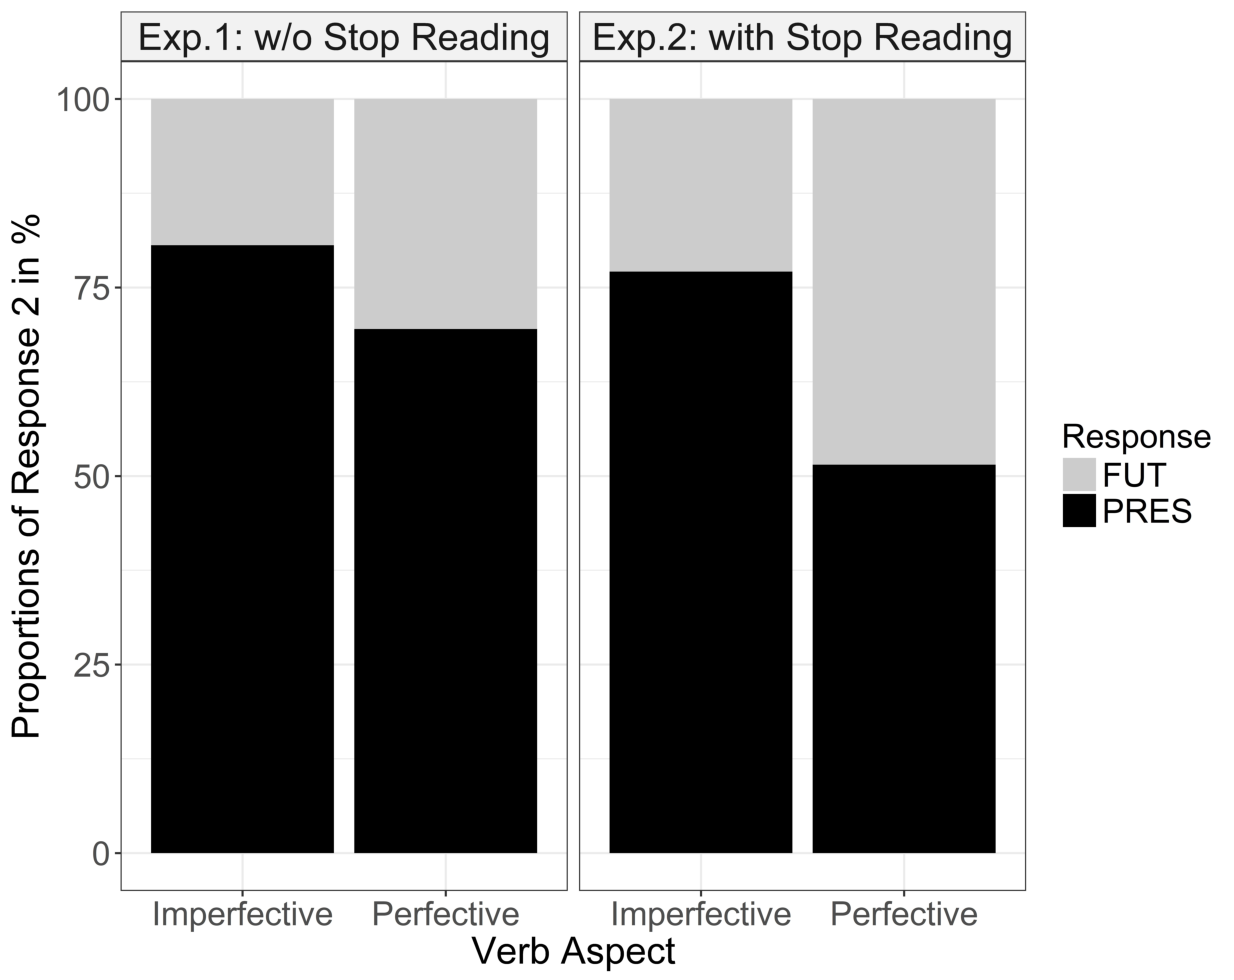
\includegraphics[height=.4\textheight]{figures/06gattnar_etal_fig1.pdf}
\caption{Response 2 (present versus future) in Experiments 1 and 2 as a function of verb aspect}
\label{fig:eins}
\end{figure}

\subsubsection{Early versus late responses in Experiment 2}

\figref{fig:zwei} shows how valid localizations in time accumulate across the regions of target sentences with \textsc{ipv} (left panel) and \textsc{pv} verb aspect (right panel). Numbers indicate the proportions of localizations in the present within the valid responses, i.e., disregarding continuations. Whereas we recognize no trend for the \textsc{ipv} aspect, it appears that for the \textsc{pv} aspect these proportions remain around $41\%$ until they rise in the last region up to $51\%$ for Response 2. To determine whether the increase is substantial, Response 2 was categorized as Early (if it matched Response 1 given earlier than region 8) or Late (if it matched Response 1 given on region 8 or revised earlier Response 1) and was subjected to a GLMM analysis with the fixed factors Aspect and Time (Early vs. Late). The GLMM converged for random intercepts (participants and items) and random slopes for Aspect (items). In addition to a strong effect of Aspect, Aspect interacted with Time [Asp: $z=3.61$\textup{***}; Asp${}\times{}$Time: $z=3.40$\textup{***}]. We take this interaction to show that the proportion of localizations in the present is indeed substantially larger for late compared to early responses in case of a \textsc{pv} aspect ($71$ vs. $41\%$; total $n$: $91$ vs. $177$); no such difference is obtained in case of an \textsc{ipv} aspect ($74$ vs. $78\%$; total $n$: $89$ vs. $181$).

\begin{figure}
\includegraphics[height=.4\textheight]{figures/06gattnar_etal_fig2.pdf}
\caption{Responses 1 and 2 in Experiment 2 as a function of aspect dependent on sentence position}
\label{fig:zwei}
\end{figure}

In sum, the results substantiate the claim that the \textsc{pv} aspect on a \isi{speech act verb} reduces its \isi{performative} force compared to the \textsc{ipv} aspect, i.e., it reduces the probability that a native speaker interprets the sentence containing it as to perform a \isi{speech act}. However, the \isi{performative} force of the verb is often preserved nevertheless, in that speakers frequently interpret the utterance of the sentence as a \isi{speech act}. In addition, given a \textsc{pv} verb aspect, there is evidence that speakers more likely opt for a \isi{speech act} interpretation after having processed the uttered sentence as a whole. This claim is supported by much more \isi{speech act} interpretations in Experiment 1 without \textsc{Stop-Reading} than in Experiment 2 with \textsc{Stop-Reading}; further evidence comes from Experiment 2 in which \isi{speech act} interpretations were more frequent if participants read the whole sentence compared to when they stopped reading before the end of the sentence. This might be taken to indicate that the aspect morphology of the sentence initial \textsc{pv} verb is in conflict with a \isi{speech act} interpretation, with the latter prevailing in particular if based on a full interpretation of the sentence. In line with this, we observe that a valid Response 1 often persists in Response 2 in particular for localizations in the present, $95\%$, compared to localizations in the future, $82\%$.

\section{Discussion and outlook}\label{sct:drei}

The results of the experiments confirm our hypothesis that \textsc{pv} \isi{speech act} verbs can be used in \isi{performative} utterances, and may in principle substitute the \textsc{ipv} \isi{speech act} verbs. Our investigation does not explain the restrictions of the class of \textsc{pv} verbs that can occur in \isi{performative} utterances. Like \citet{Wiemer2014} we tend to the opinion that \textsc{pv} performatives are lexicalized to a certain extent. For our investigation the evidence that \textsc{pv} \isi{speech act} verbs are interpreted as \isi{present tense} verbs is the most important result. In both experiments taken together about $60\%$ of the \textsc{pv} \isi{speech act} verbs were interpreted as present \isi{perfective}. As not all of our \isi{speech act} verbs were \textit{verba dicendi} (for example ‘to thank’, ‘to invite’, ‘to welcome’, etc.), we may conclude, that not only \textit{verba dicendi} but also other \isi{speech act} verbs can be used in \isi{performative speech} acts. Following our hypothesis, we have strong evidence that the present \isi{perfective} \isi{speech act} verbs own \isi{performative} force. This is shown by the frequent \isi{present tense} localizations of events denoted by our \textsc{pv} \isi{speech act} verbs. Localization based on the full sentences promoted the localizations of the \textsc{pv} performatives in the \isi{present tense}. We infer this from the comparison of the two experiments. Moreover, we found a late increase of locations in the \isi{present tense} in Experiment 2 and a persistence of early localizations in the present. Therefore, we conclude that the sentence context plays an important role for the temporal localizations in the case of \textsc{pv} \isi{speech act} verbs. The verbal aspect is thus not the decisive factor for the well-formedness of \isi{performative} utterances in \ili{Russian}. The interpretation as \isi{performative} is also influenced by the particular \isi{semantics} of the \isi{speech act} verbs, the sentence embedding the \isi{speech act verb}, and maybe the preceding context.

Summing up, we reach the following conclusions, which are in part preliminary and need further support:

First, \textsc{pv} \isi{speech act} verbs can be used in \isi{performative speech} acts, because, due to the available \isi{present tense} interpretation, they fulfill condition ‘\isi{present tense}’ that is inevitable to carry out a \isi{performative speech act}. Second, the information conveyed by the sentence information following the \textsc{pv} \isi{speech act verb} has an influence on the interpretation of the verb if it bears \textsc{pv} but not \textsc{ipv} aspect. Third, given the very low ratings of \textsc{pv} performatives without preceding context (see footnote \ref{fn5}), we suspect that the \isi{speech act} interpretation also benefits from the preceding context. Evidence for this comes from the fact that the results with \textsc{pv} verbs in Experiment 2 increase in late present localization nearly to the rates for the \textsc{ipv} verbs. In the case of \textsc{pv} \isi{speech act} verbs, we can even speak of an interaction between the successive enhancement of context information and the localization in the present. The \textsc{pv} \isi{speech act verb} by itself may be crucial for present localization, but a more reliable localization is reached when the \isi{speech act verb} is embedded in a wider context. The stronger \isi{performative} power of the \textsc{pv} aspect in Experiment 1, where the whole \isi{speech act} appeared before the decision, confirms how the quantity of the sentence information has influence on the decision.

As far as we know, this is the first experimental investigation on aspect use in \ili{Russian} performatives showing that \textsc{pv} \isi{speech act} verbs can be used in \isi{performative} utterances. A next step would be to answer the question, whether and how the use of \textsc{pv} \isi{speech act} verbs influences the sentence meaning in comparison to \textsc{ipv} \isi{speech act} verbs.  Like \citeauthor{Israeli2001} we tend to hypothesize a pragmatic difference between \textsc{ipv} and \textsc{pv} \isi{performative} utterances; see example \REF{ex:item}. It would be interesting to check whether an overt subject even strengthens the marking of authority in \isi{performative} utterances. Another important consideration is the verbal \isi{semantics} of \textsc{ipv} and \textsc{pv} \isi{speech act} verbs. When we argue with \citet{Breu1980} and \citet{Dewit2017}, we must also look at the verb immanent \isi{aspectual} functions in which \textsc{ipv} and \textsc{pv} \isi{speech act} verbs are different from each other. Following this line of reasoning, \textsc{ipv} \isi{speech act} verbs would name and perform the \isi{performative} event, whereas a \textsc{pv} \isi{speech act} would emphasize the completion of the \isi{performative speech act}. Both approaches are well worth pursuing and will give motivate further experimental investigation.


\section*{Abbreviations}

\begin{tabularx}{.5\textwidth}{@{}lQ@{}}
\textsc{1}&1st person\\
\textsc{3}&3rd person\\
\textsc{dat}&{dative}\\
\textsc{ipv}&{imperfective aspect}\\
\textsc{neg}&{negation}\\
\textsc{past}&{past tense}\\
\end{tabularx}%
\begin{tabularx}{.5\textwidth}{@{}lQ@{}}
\textsc{pl}&{plural}\\
\textsc{pres}&{present tense}\\
\textsc{ptcl}&particle\\
\textsc{pv}&{perfective aspect}\\
\textsc{RNC}&{Russian} National Corpus\\
\textsc{sg}&singular\\
\end{tabularx}

\section*{Acknowledgements}
Special thanks go to Prof. Tatiana V. Chernigovskaya, head of the Laboratory for Cognitive Studies, St. Petersburg State University and her staff member Daria Chernova. They supported us in recruiting participants and placed a laboratory to our disposal for conducting the experiments. Furthermore, we wish to thank Tilman Berger, Stefan Heck, Eugen Kravchenko, Inna Pirina, Tatiana Pere\-voz\-chi\-kova and two anonymous reviewers for their helpful comments.

% \section*{Appendix}\label{appendix}
% \small{
% \begin{enumerate}

% \item\begin{labeling}{c} %1
% \item[c] Дима плохо себя ведёт на уроке. Учительница делает ему замечание. Он говорит:
% \newline\textit{Dima plocho sebja vedёt na uroke. Učitel’nica delaet emu zamečanie. On govorit:}
% \newline‘Dima behaves badly during the lesson. The teacher makes him a remark. He says:’

% \item[t] Извинюсь/Извиняюсь за своё поведение, я больше так не буду.
% \newline\textit{Izvinjus’/Izvinjajus’ za svoё povedenie, ja bol’še tak ne budu.}
% \newline‘I apologize\textsc{.pv/ipv} for my behavior, I will not do it again.’
% \end{labeling}

% \item\begin{labeling}{c} %2
% \item[c] Анна учится в пятом классе. Сегодня они начали новую тему по математике и получили домашнее задание. Анна не понимает, что делать, и говорит своей старшей сестре:
% \newline\textit{Anna učitsja v pjatom klasse. Segodnja oni načali novuju temu po matematike i polučili domašnee zadanie. Anna ne ponimaet, čto delat’, i govorit svoej staršej sestre:}
% \newline‘Anna studies in 5\textsuperscript{th} grade. Today they started a new topic in maths and received homework. Anna doesn’t understand what to do and says to her older sister:’

% \item[t] Попрошу/Прошу тебя помочь мне с моим домашним заданием по математике!
% \newline\textit{Poprošu/Prošu tebja pomoč’ mne s moim domašnim zadaniem po matematike!}
% \newline‘I ask\textsc{.pv/ipv} you to help me with my maths homework!’
% \end{labeling}

% \item\begin{labeling}{c} %3
% \item[c] Инспектор заметил значительные недостатки у контрольной партии товара. Он заявляет об этом в письменной форме и в конце документа добавляет:
% \newline\textit{Inspektor zametil značitel’nye nedostatki u kontrol’noj partii tovara. On zajavljaet ob ėtom v pis’mennoj forme i v konce dokumenta dobavljaet:}
% \newline‘The inspector noticed significant shortcomings in the control lot of the goods. He declares this in written form and at the end of the document adds:’

% \item[t] Потребую/Требую существенного повышения качества вашего товара в кратчайшие сроки.
% \newline\textit{Potrebuju/Trebuju suščestvennogo povyšenija kačestva vašego tovara v kratčajšie sroki.}
% \newline‘I demand\textsc{.pv/ipv} a substantial improvement in the quality of your goods in the shortest time.’
% \end{labeling}

% \item\begin{labeling}{c} %4
% \item[c] Г-жа Смирнова встречает около дома своих соседей. Они загружают многочисленные чемоданы в машину. Г-жа Смирнова узнает, что они едут в отпуск. Она прощается:
% \newline\textit{G-ža Smirnova vstrečaet okolo doma svoich sosedej. Oni zagružajut mnogočislennye čemodany v mašinu. G- ža Smirnova uznaet, čto oni edut v otpusk. Ona proščaetsja:}
% \newline‘Ms. Smirnova meets her neighbors next to her house. They load numerous suitcases into the car. Ms. Smirnova finds out that they are going on vacation. She says goodbye:’

% \item[t] Пожелаю/Желаю вам счастливого пути, хорошей погоды и замечательного отпуска!
% \newline\textit{Poželaju/Želaju vam sčastlivogo puti chorošej pogody i zamečatel’nogo otpuska!}
% \newline‘I wish\textsc{.pv/ipv} you a happy journey, good weather and a wonderful vacation.’
% \end{labeling}

% \item\begin{labeling}{c} %5
% \item[c] Мария должна отменить встречу со своими подругами. Подруги договариваются сразу на следующий день, а Мария говорит:
% \newline\textit{Marija dolžna otmenit’ vstreču so svoimi podrugami. Podrugi dogovarivajutsja srazu na sledujuščij den’, a Marija govorit:}
% \newline‘Maria must cancel the meeting with her friends. The girlfriends agree immediately on the next day, and Maria says:’

% \item[t] Поблагодарю/Благодарю вас, мои любимые и верные подруги, за ваше понимание.
% \newline\textit{Poblagodarju/\ili{Blagodarju} vas, moi ljubimye i vernye podrugi, za vaše ponimanie.}
% \newline‘I thank\textsc{.pv/ipv} you, my dear and faithful friends, for your understanding.’
% \end{labeling}

% \item\begin{labeling}{c} %6
% \item[c] В школе состоялся шахматный турнир. В финале Витя проиграл Алине и сказал ей:
% \newline\textit{V škole sostojalsja šachmatnyj turnir. V finale Vitja proigral Aline i skazal ej:}
% \newline‘A chess tournament took place at school. In the final, Vitja lost to Alina and said to her:’

% \item[t] Признáю/Признаю́ тебя заслуженной победительницей, ты очень хорошо играешь!
% \newline\textit{Priznáju/Priznajú tebja zaslužennoj pobeditel’nicej ty očen’ chorošo igraeš’!}
% \newline‘I recognize\textsc{.pv/ipv} you as a well-deserved winner, you play very well!’
% \end{labeling}

% \item\begin{labeling}{c} %7
% \item[c] Вере предлагают новую должность на работе. Она долго колеблется, но её начальник говорит:
% \newline\textit{Vere predlagajut novuju dolžnost’ na rabote. Ona dolgo kolebletsja, no eё načal’nik govorit:}
% \newline‘Vera is offered a new position at work. She hesitates for a long time, but her boss says:’

% \item[t] Уверю/Уверяю Вас, что эта должность – важный шаг на пути к успеху.
% \newline\textit{Uverju/Uverjaju Vas, čto ėta dolžnost’ – važnyj šag na puti k uspechu.}
% \newline‘I assure\textsc{.pv/ipv} you that this position is an important step on the way to success.’
% \end{labeling}

% \item\begin{labeling}{c} %8
% \item[c] Солдаты отказываются выполнять приказ своего командира. Он предупреждает их о последствиях и говорит:
% \newline\textit{Soldaty otkazyvajutsja vypolnjat’ prikaz svoego komandira. On predupreždaet ich o posledstvijach i govorit:}
% \newline‘The soldiers refuse to carry out the order of their commander. He warns them about the consequences and says:’

% \item[t] Я oчень рассержен, и прикажу/приказываю вам в самый последний раз!
% \newline\textit{Ja očen’ rasseržen, i prikažu/prikazyvaju vam v samyj poslednij raz!}
% \newline‘I am very angry, and I order\textsc{.pv/ipv} you for the very last time!’
% \end{labeling}

% \item\begin{labeling}{c} %9
% \item[c] Фёдор уже давно влюблен в свою одноклассницу. Он провожает её до её дома и говорит:
% \newline\textit{Fёdor uže davno vljublen v svoju odnoklassnicu. On provožaet eё do eё doma i govorit:}
% \newline‘Fedor has been in love with his classmate for a long time. He escorts her to her house and says:’

% \item[t] Признáюсь/Признаю́сь, что я уже очень давно и безнадёжно в тебя влюблён.
% \newline\textit{Priznájus’/Priznajús’ čto ja uže očen’ davno i beznadёžno v tebja vljublёn.}
% \newline‘I admit\textsc{.pv/ipv} that I have been hopelessly in love with you for a very long time.’
% \end{labeling}

% \item\begin{labeling}{c} %10
% \item[c] Ира и Максим недавно переселились в новую квартиру. В подъезде Ира встречает своего нового соседа, и так как они планируют праздник, она говорит ему:
% \newline\textit{Ira i Maksim nedavno pereselilis’ v novuju kvartiru. V pod”ezde Ira vstrečaet svoego novogo soseda, i tak kak oni planirujut prazdnik, ona govorit emu:}
% \newline‘Ira and Maxim recently moved into a new apartment. At the entrance, Ira meets her new neighbor, and since they plan a party, she tells him:’

% \item[t] Приглашу/Приглашаю Вас к нам на праздничный ужин по поводу нашего новоселья!
% \newline\textit{Priglašu/Priglašaju Vas k nam na prazdničnyj užin po povody našego novosel’ja!}
% \newline‘I invite\textsc{.pv/ipv} you to our place for a festive housewarming dinner!’
% \end{labeling}

% \item\begin{labeling}{c} %11
% \item[c] Саша не хочет идти спать. Он пытается убедить свою маму, что может ложиться спать чуть позже. Наконец, она соглашается и говорит:
% \newline\textit{Saša ne chočet idti spat’. On pytaetsja ubedit’ svoju mamu, čto možet ložit’sja spat’ čut’ pozže. Nakonec, ona soglašaetsja i govorit:}
% \newline‘Sasha does not want to go to sleep. He tries to convince his mother that he can go to bed a little later. Finally, she agrees and says:’

% \item[t] Разрешаю/Разрешу тебе почитать, но через полчаса ты пойдёшь спать.
% \newline\textit{Razrešaju/Razrešu tebe počitat’, no čerez polčasa ty pojdёš’ spat’.}
% \newline‘I allow\textsc{.pv/ipv} you to read, but in half an hour you'll go to sleep.’
% \end{labeling}

% \item\begin{labeling}{c} %12
% \item[c] Лиза хочет съехать со своей квартиры. При разговоре с хозяином обсуждаются окончательные детали. Лиза уверяет хозяина:
% \newline\textit{Liza chočet s’’echat’ so svoej kvartiry. Pri razgovore s chozjainom obsuždajutsja okončatel’nye detali. Liza uverjaet chozjaina:}
% \newline‘Lisa wants to move out of her apartment. In the conversation with the owner, the final details are discussed. Lisa assures the owner:’

% \item[t] Обязываюсь/Обяжусь сделать в квартире ремонт, но мне нужна Ваша помощь.
% \newline\textit{Objazyvajus’/Objažus’ sdelat’ v kvartire remont, no mne nužna Vaša pomošč’.}
% \newline‘I commit\textsc{.pv/ipv} myself to make repairs in the apartment, but I need your help.’
% \end{labeling}

% \item\begin{labeling}{c} %13
% \item[c] После того как несколько крупных компаний предложили значительные суммы, бизнесмен благодарит их за интерес и говорит:
% \newline\textit{Posle togo kak neskol’ko krupnych kompanij predložili značitel’nye summy, biznesmen blagodarit ich za interes i govorit:}
% \newline‘After several large companies offered significant sums, the businessman thanks them for their interest and says:’

% \item[t] Ваше предложение я отклоняю/отклоню, такие условия мне не подходят.
% \newline\textit{Vaše predloženie ja otklonjaju/otklonju, takie uslovija mne ne podchodjat.}
% \newline‘I reject\textsc{.pv/ipv} your proposal, such conditions do not suit me.’
% \end{labeling}

% \item\begin{labeling}{c} %14
% \item[c] Катя выигрывает теннисный турнир, и журналист берёт у неё интервью. Прежде всего он приветствует её и говорит:
% \newline\textit{Katja vyigryvaet tennisnyj turnir, i žurnalist berёt u neё interv’ju. Prežde vsego on privetstvuet eё i govorit:}
% \newline‘Katja wins a tennis tournament and a journalist takes an interview with her. First of all, he greets her and says:’

% \item[t] Первым делом поздравляю/поздравлю Вас с вашей очередной эффектной победой!
% \newline\textit{Pervym delom pozdravljaju/pozdravlju Vas s vašej očerednoj ėffektnoj pobedoj!}
% \newline‘First of all, I congratulate\textsc{.pv/ipv} you on another spectacular victory!’
% \end{labeling}

% \item\begin{labeling}{c} %15
% \item[c] На выпускной церемонии в конце года София получает награду за отличные оценки. Учитель вручает ей грамоту со словами:
% \newline\textit{Na vypusknoj ceremonii v konce goda Sofija polučaet nagradu za otličnye ocenki. Učitel’ vručaet ej gramotu so slovami:}
% \newline‘At the graduation ceremony at the end of the year, Sofia receives the award for excellent grades. The teacher hands her a letter with the words:’

% \item[t] Хвалю/Похвалю тебя, София, ты одна из лучших учениц школы!
% \newline\textit{Chvalju/Pochvalju tebja Sofija, ty odna iz lučšich učenic školy!}
% \newline‘I praise\textsc{.pv/ipv} you, Sofia, you are one of the best pupils of the school!’
% \end{labeling}

% \item\begin{labeling}{c} %16
% \item[c] Борис разговаривает со своей матерью и просит совета. Он рассказывает о проблемах с женой и сознаётся, что думает о разводе. Тогда мать говорит ему:
% \newline\textit{Boris razgovarivaet so svoej mater’ju i prosit soveta. On rasskazyvaet o problemach s ženoj i soznaёtsja, čto dumaet o razvode. Togda mat’ govorit emu:}
% \newline‘Boris talks with his mother and asks for advice. He talks about problems with his wife and confesses that he is thinking about a divorce. Then the mother says to him:’

% \item[t] Предупреждаю/Предупрежу, после вашего развода назад дороги уже не будет!
% \newline\textit{Predupreždaju/Preduprežu, posle vašego razvoda nazad dorogi uže ne budet!}
% \newline‘I warn\textsc{.pv/ipv} you, after your divorce, there will be no more way back!’
% \end{labeling}

% \item\begin{labeling}{c} %17
% \item[c] Антон приводит свою девушку на семейный праздник. В начале праздника он говорит своей семье:
% \newline\textit{Anton privodit svoju devušku na semejnyj prazdnik. V načale prazdnika on govorit svoej sem’e:}
% \newline‘Anton takes his girlfriend to a family holiday. At the beginning of the holiday, he tells his family:’

% \item[t] Представляю/Представлю вам мою девушку, её зовут Света Смирнова.
% \newline\textit{Predstavljaju/Predstavlju vam moju devušku, её zovut Sveta Smirnova.}
% \newline‘I introduce\textsc{.pv/ipv} to you my girlfriend, she is called Sveta Smirnova.’
% \end{labeling}

% \item\begin{labeling}{c} %18
% \item[c] Анна разбила вазу, которую её маме подарили подруги. Она плачет и просит у мамы прощения. Мама улыбается и говорит:
% \newline\textit{Anna razbila vazu, kotoruju eё mame podarili podrugi. Ona plačet i prosit u mamy proščenija. Mama ulybaetsja i govorit:}
% \newline‘Anna broke a vase that friends gave to her mother. She cries and asks her mother for forgiveness. The mother smiles and says:’

% \item[t] Я тебя прощаю/прощу, эта ужасная ваза мне никогда не нравилась.
% \newline\textit{Ja tebja proščaju/prošču, ėta užasnaja vaza mne nikogda ne nravilas’.}
% \newline‘I forgive\textsc{.pv/ipv} you, I never liked this terrible vase.’
% \end{labeling}

% \item\begin{labeling}{c} %19
% \item[c] Алексей должен показать представителям нескольких других компаний помещения своего предприятия. Он начинает экскурсию со словами:
% \newline\textit{Aleksej dolžen pokazat’ predstaviteljam neskol’kich drugich kompanij pomeščenija svoego predprijatija. On načinaet ėkskursiju so slovami:}
% \newline‘Alexej should show representatives of several other companies the premises of his company. He begins the tour with the words:’

% \item[t] Приветствую/ Поприветствую Вас и предлагаю начать нашу небольшую экскурсию по предприятию.
% \newline\textit{Privetstvuju/Poprivetsvuju Vas i predlagaju načat’ našu nebol’šuju ėkskursiju po predprijatiju.}
% \newline‘I welcome\textsc{.pv/ipv} you and suggest that we begin our small excursion around the company.’
% \end{labeling}

% \item\begin{labeling}{c} %20
% \item[c] Сотрудник большой фирмы забыл свой пропуск дома. На работе охранник не позволяет ему войти в помещение и говорит:
% \newline\textit{Sotrudnik bol’šoj firmy zabyl svoj propusk doma. Na rabote ochrannik ne pozvoljaet emu vojti v pomeščenie i govorit:}
% \newline‘A large company employee forgot his pass at home. At work, the guard does not allow him to enter the room and says:’

% \item[t] Я отказываю/откажу Вам в допуске, Вы не можете войти без пропуска.
% \newline\textit{Ja otkazyvaju/otkažu Vam v dopuske, Vy ne možete vojti bez propuska.}
% \newline‘I refuse\textsc{.pv/ipv} you permission, you cannot enter without a pass.’
% \end{labeling}
% \end{enumerate}
% }

\sloppy
\printbibliography[heading=subbibliography,notkeyword=this]
\end{document}
